
\makeatletter
\if@twocolumn
	\def\cybershakesize{0.9\columnwidth}
\else
	\def\cybershakesize{0.5\textwidth}
\fi
\makeatother


\begin{figure}[ht!]
    \centering
    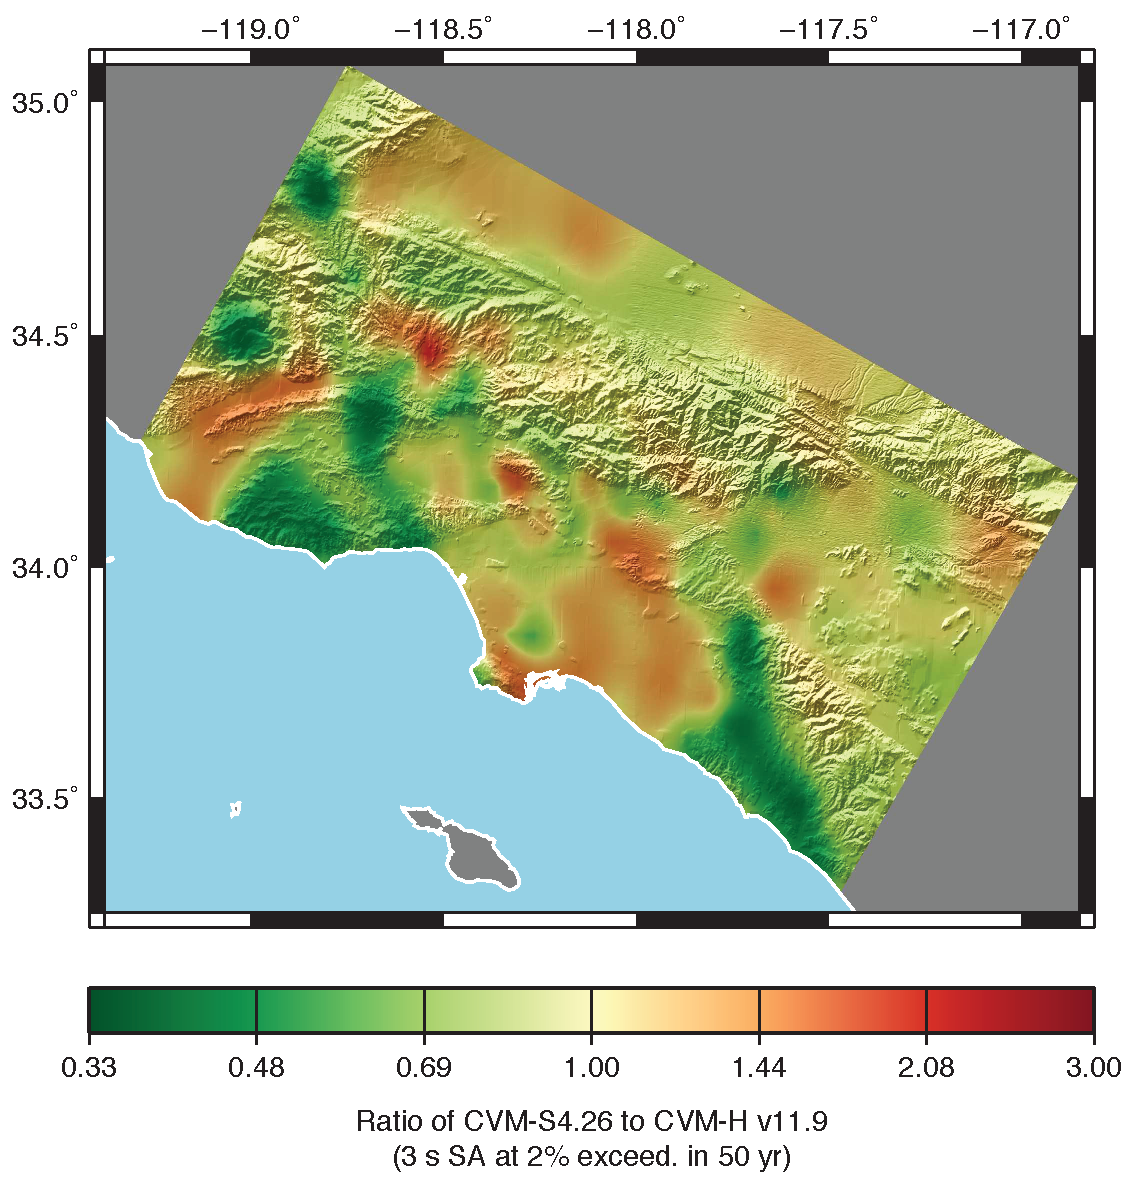
\includegraphics
        [width=\cybershakesize]
        {figures/pdf/cybershake}
    \caption{Ratio between two CyberShake seismic hazard maps obtained using two different velocity models, CVM-S4.26 and CVM-H. The underlying hazard maps correspond to a 3-seconds spectral acceleration with a 2\% chance of exceedance in 50 years. The discrete regular grids used as input for these computations were built using UCVM meshing utilities.}
    \label{fig:cybershake}
\end{figure}

